\documentclass{article}
\documentclass[a4paper,12pt, italian]{article}
\usepackage{geometry}
\geometry{a4paper, top=3cm, bottom=3cm, left=3cm, right=3cm, heightrounded, bindingoffset=5mm}
\usepackage[italian]{babel}
\usepackage[version=3]{mhchem} 
\usepackage{siunitx} 
\usepackage{graphicx}
\usepackage{natbib} 
\usepackage{amsmath}
\usepackage{hyperref}
%\usepackage[labelformat=empty]{caption}
\setlength\parindent{15pt}
\usepackage{natbib}
\usepackage{amscd}
\usepackage{siunitx}
\usepackage{booktabs}
\usepackage{multicol}
\usepackage{tikz}
\usepackage{amsmath,amssymb}
\usepackage{amsthm}
\usepackage{tikz}
\usepackage{cancel}
\usepackage{placeins} %aggiungi questo package e usa \FloatBarrier all'inizio e alla fine della sequenza di tabelle
\usepackage[labelsep=space]{caption} 
\renewcommand{\labelenumi}{\alph{enumi}.} 
\newcommand{\minitab}[2][l]{\begin{tabular}#1 #2\end{tabular}}

\title{\textsc{Studio delle leggi dell'ottica tramite il fenomeno dell'interferenza}}

\author{Laura \textsc{Trombetta}\\ Alessandro Maria \textsc{Turturiello}\\Federico \textsc{Venturoli}} 



\begin{document}

\maketitle 

\begin{center}
\begin{tabular}{l r}
Eseguita il giorno: &  17 marzo 2022 \\ 
Gruppo T2A-4: & Trombetta Laura\\
& Turturuello Alessandro Maria \\
& Venturoli Federico \\ 

\end{tabular}
\end{center}
\begin{abstract}
    Lo scopo della presente relazione è quello di esporre i metodi sperimentali utilizzati durante l'esperienza riguardante i fenomeni di interferenza luminosa. Inoltre, tramite questo fenomeno si è in grado, tramite le relazioni espresse dalle equazioni \ref{aria} e \ref{eq 3}, di ricavare l'indice di rifrazione dell'aria e del vetro.
\end{abstract}
\tableofcontents
\maketitle
\newpage

\section{Introduzione teorica e descrizione dell'apparato sperimentale}
Le misure sono state raccolte con due configurazioni ottiche differenti. 
\begin{figure}[h!]
    \centering
    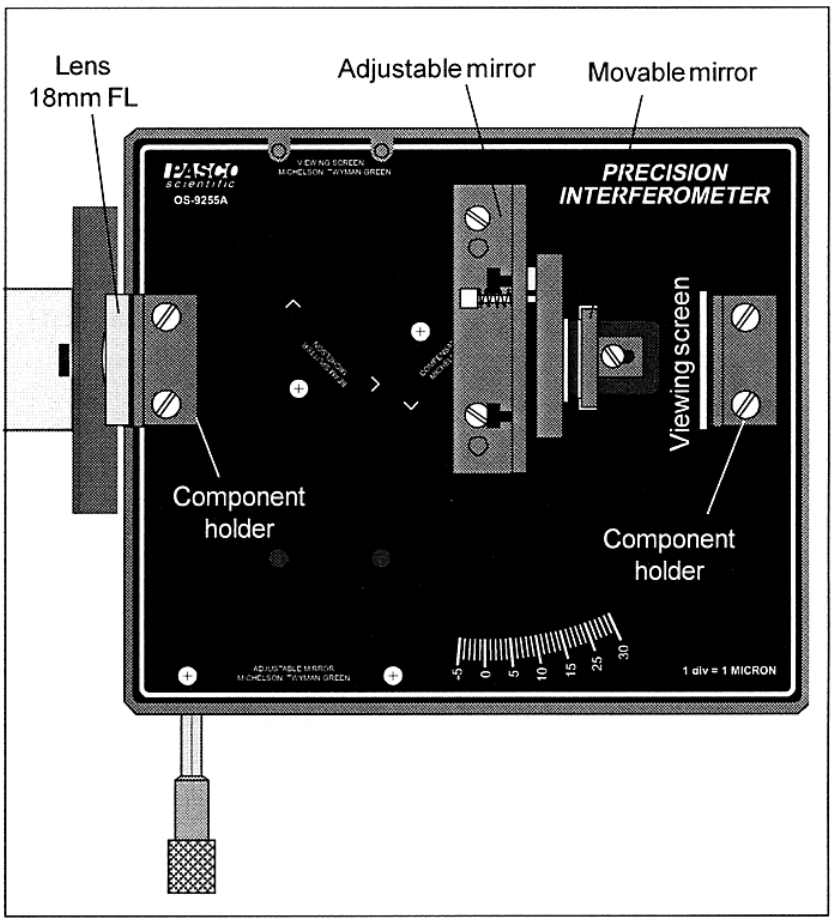
\includegraphics[scale=.45]{immagini/faby pero.png}
    \caption{Configurazione di Fabry-Perot}
    \label{fabi pero}
\end{figure}
In primis abbiamo operato con il sistema ottico di \textit{Fabry-Perot}. L'apparato rappresentato in Figura \ref{fabi pero} è costituito da una base con le indicazioni per posizionare correttamente le lenti necessarie durante l'esperienza; una lente convergente da $18\,mm$, specchi (uno mobile e uno fisso) e un nonio, necessario per regolare in maniera precisa la distanza tra lo specchio fisso e quello mobile. Esterno alla base abbiamo posizionato il banco ottico con la sorgente laser (rosso), allineandolo agli specchi e alle lenti.

In questa configurazione la luce proveniente dalla sorgente laser è posizionata in modo tale che il fascio incida perpendicolarmente allo specchio nel centro e ritorni coincidente con la sorgente. Il raggio è soggetto al fenomeno dell'interferenza, reso visibile grazie alla presenza della lente che lo fa divergere.

Un'interferenza si verifica quando in un punto dello spazio due o più onde si sommano in modo coerente, caratterizzando l'onda risultante con massimi e minimi di ampiezza, e quindi di intensità. Questi ultimi non necessariamente coincidono con le somme dei massimi e minimi delle onde originarie.

Nella nostra esperienza l'interferenza si manifesta tramite dei cerchi concentrici luminosi proiettati su una superficie posta ad almeno un metro di distanza.

Nella configurazione di \textit{Fabry-Perot} si crea una figura di interferenza data da una doppia riflessione del raggio tra i due specchi, che permette di ottenere un effetto simile a quello che si avrebbe in presenza di più sorgenti luminose.

Nella cavità il raggio resta in parte indeviato e viene in parte riflesso raggiungendo lo schermo con uno sfasamento $\delta_r$ che dipende dalla differenza di cammino ottico; cambiando la distanza tra i due specchi, infatti, si osserva lo scorrimento delle frange di interferenza. 

La differenza di fase $\delta$ non tiene conto solo del differente cammino ottico ma anche di uno sfasamento, nel nostro caso considerato trascurabile. Si presenta un'interferenza costruttiva quando la differenza di fase è data da
$$
\delta=2N\pi 
$$
ovvero quando si sommano in fase le ampiezze delle due onde. Si può, quindi, descrivere la figura di interferenza attraverso la relazione
\begin{equation}
    \delta_r \dfrac{\lambda}{2\pi}+2\cdot\cos\theta=N\lambda
\end{equation}
dove $\lambda$ è la lunghezza d'onda del laser, il quale nel nostro caso è a He-Ne e ha $\lambda=632.8\,nm$, mentre $\theta$ è l'angolo ottenuto dalla relazione 
$$
\cos\theta=\dfrac{r}{D}
$$
dove $r$ è la distanza rispetto al centro della figura di interferenza del massimo che si utilizza come riferimento e $D$ è la distanza tra la sorgente dell'interferenza e lo schermo rilevatore.
\begin{figure}[h!]
    \centering
    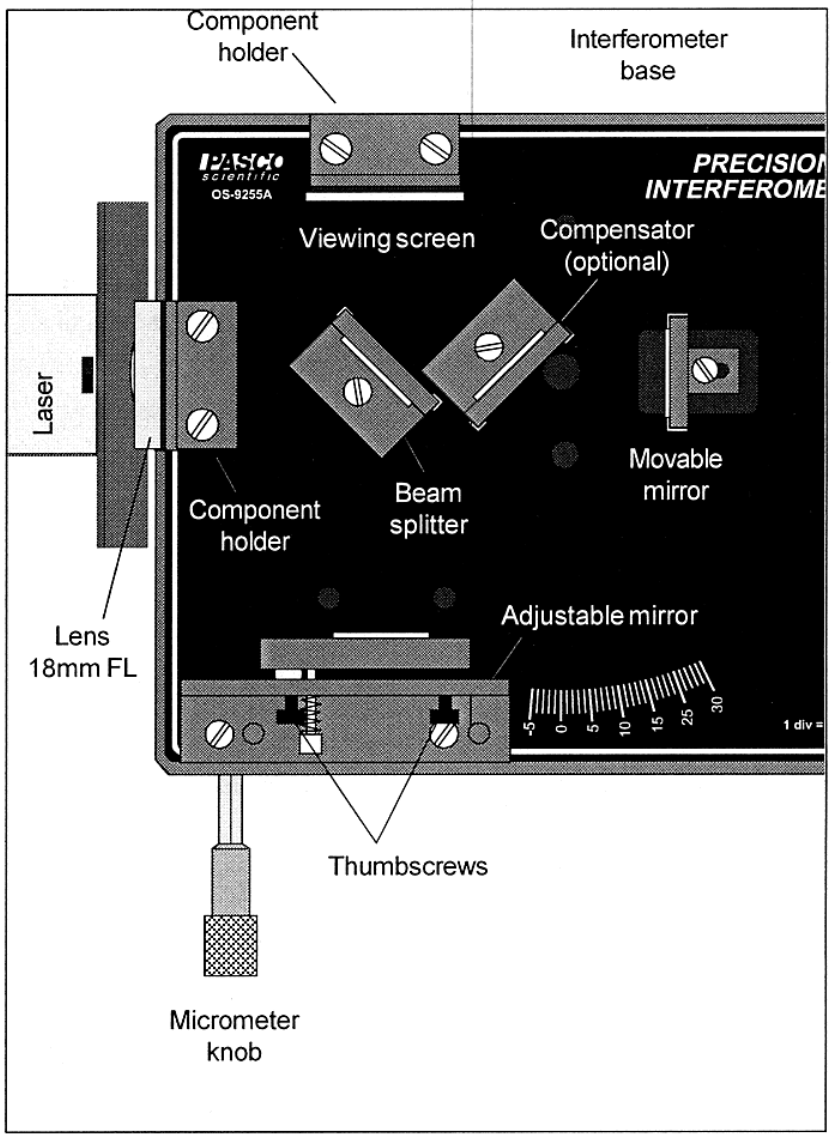
\includegraphics[scale=.37]{immagini/michaelson.png}
    \caption{Configurazione di Michelson}
    \label{michelino}
\end{figure}
Lo scopo di questa parte di esperienza è, perciò, quello di verificare la legge e, dopo aver calibrato il nonio, determinare la lunghezza d'onda di un secondo laser di $\lambda$ ignota.
\\

In secondo luogo abbiamo operato con la configurazione di \textit{Michelson}. In maniera analoga a quella illustrata precedentemente abbiamo allineato il banco ottico, modificando però la posizione degli specchi. Abbiamo utilizzato questa configurazione per determinare l'indice di rifrazione dell'aria e quello del vetro. Nel primo caso ci siamo serviti di una pompa in grado di creare una differenza di pressione all'interno della cella; nel secondo caso abbiamo, invece, fatto uso di uno strumento che ci permettesse di ruotare una lastra di vetro, così da determinarne l'indice di rifrazione alla variazione dell'angolo di incidenza.

Nel primo caso la relazione che descrive la legge è
\begin{equation}
   \eta_{\text {aria }}=\dfrac{\Delta N\,\lambda}{2d(P_i-P_f)}
   \label{aria}
\end{equation}
mentre nel secondo caso, invece, è
\begin{equation}
\eta_{\text {vetro }}=\frac{(2 d-\Delta N \lambda)(1-\cos \theta)}{2 d \cdot(1-\cos \theta)-\Delta N \lambda}
\label{eq 3}
\end{equation}

\section{Calibrazione}
Prima di procedere con le misure dei relativi esperimenti, abbiamo ritenuto necessario compiere una verifica della calibrazione dello strumento per ottenere risultati con maggiore precisione.
Abbiamo proceduto effettuando più volte il conteggio delle frange passanti per un riferimento scelto, per uno spostamento determinato \textit{d} del nonio pari a $20\,\mu m$.

I dati ottenuti per la determinazione di $d$ attraverso le diverse misurazioni sono riportati nella Tabella \ref{tabella 1}.

Facendo uso di \textsc{ROOT} ci è stato possibile effettuare un fit dei dati, dal quale abbiamo ricavato un nuovo valore di aspettazione, indicato nell'istogramma in Figura \ref{figura 3}.
\begin{figure}[h!]
    \centering
    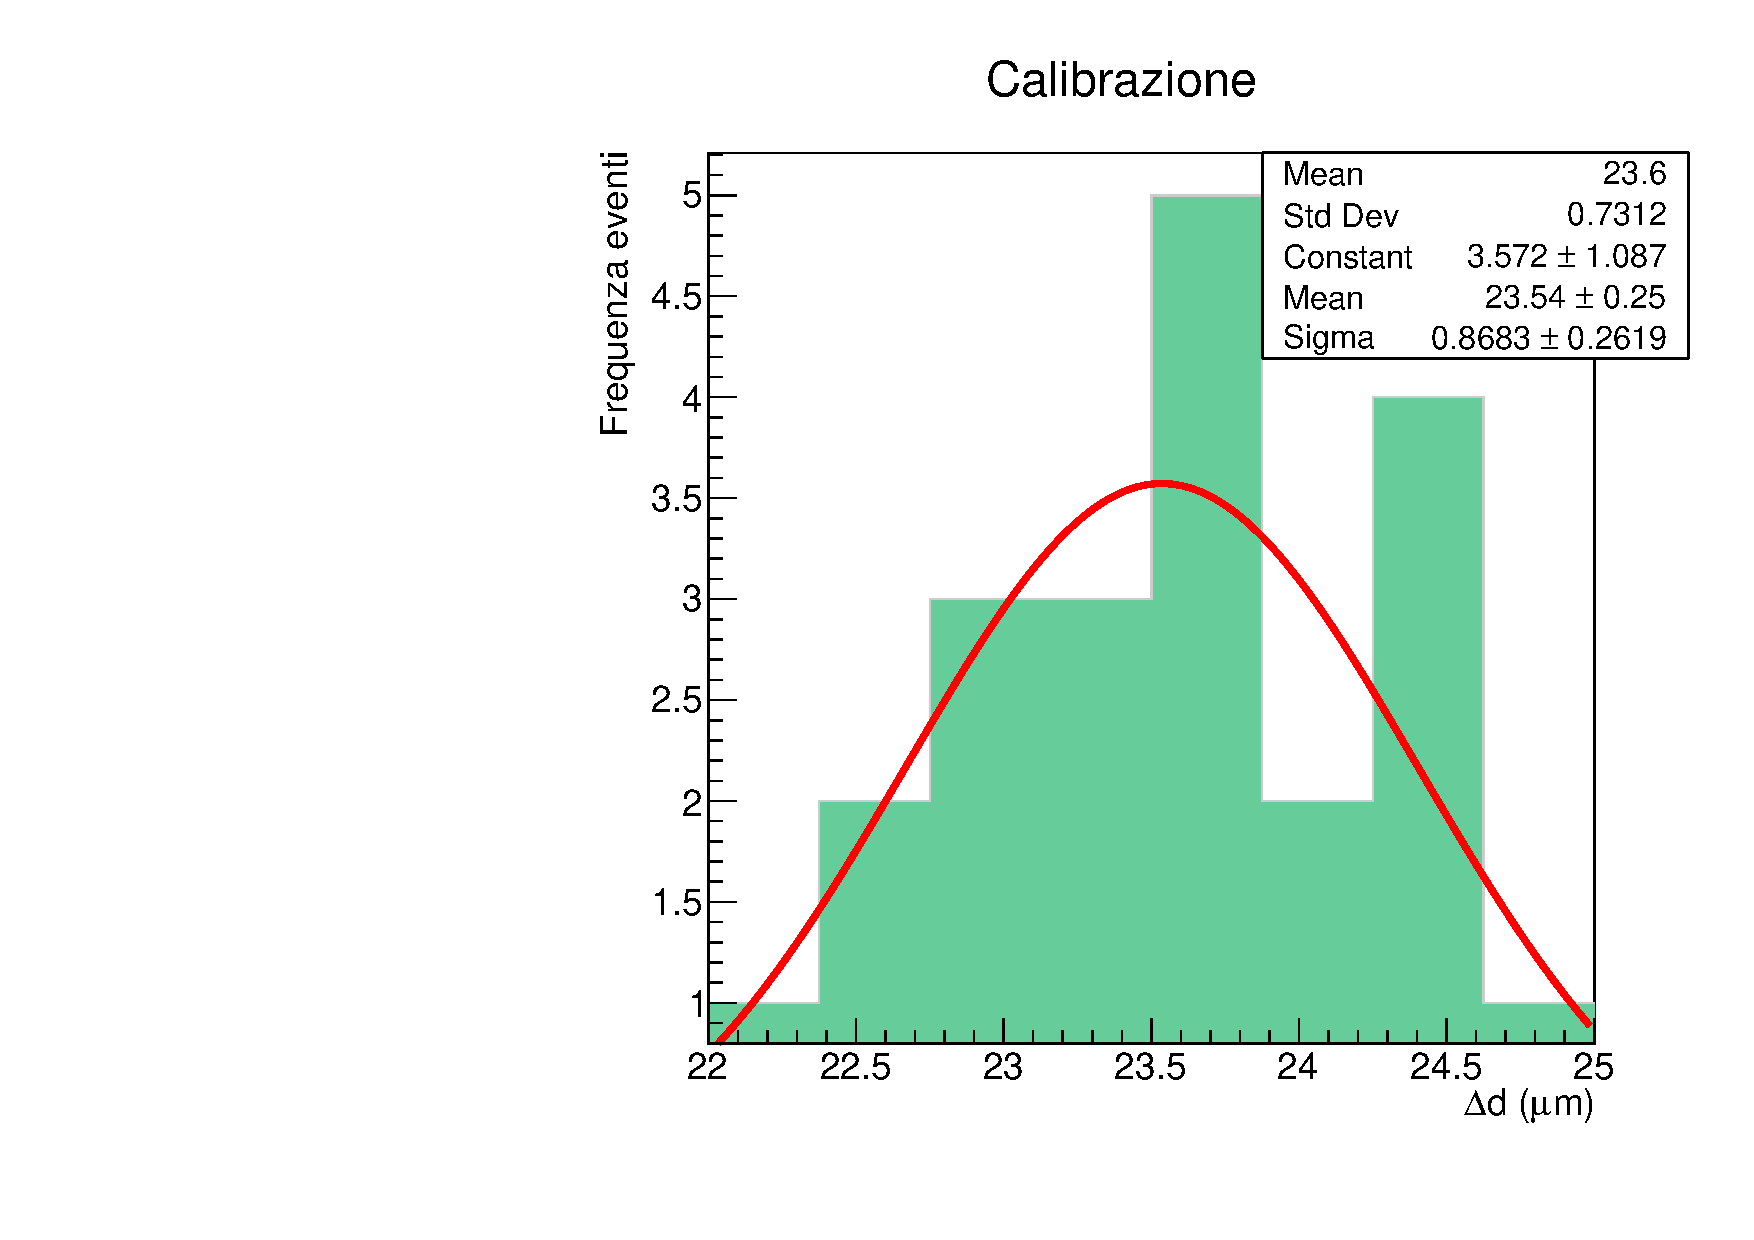
\includegraphics[scale=.35]{immagini/calibrazione nonnio.pdf}
    \caption{}
    \label{figura 3}
\end{figure}
\begin{table}[h!]
\centering
      \begin{tabular}{cc}
            & $D$ $(cm)$\\
    \hline
         & 186 \\
         & 186 \\
         & 180 \\
         & 185 \\
         & 185 \\
    \hline\hline
    & $184,4 \pm 2,51$
      \end{tabular}
      \caption{}
      \label{tabella 1}
 \end{table}

Da questo abbiamo calcolato lo scarto quadratico medio rispetto ai dati ricavati in precedenza ottenendo una deviazione standard pari a 
$$
\sigma = 0,55\, \mu m
$$


\section{Misura della lunghezza d'onda di un laser verde}
Dopo aver effettuato la calibrazione dell'apparato, ci è stato permesso testare lo strumento per la misurazione della lunghezza d'onda ignota di un secondo laser di colore verde.

Abbiamo nuovamente contato il numero di frange passanti per un riferimento scelto. Successivamente abbiamo ricavato il valore di lambda attraverso la relazione
\begin{equation}
    \lambda=\dfrac{2\cdot d\cdot \cos\theta}{N}
\end{equation}
\noindent
Le tabelle che seguono riportando i conteggi del numero di frange $\Delta N$ e il corrispondente valore $\lambda$

\begin{table}[h!]
    \centering
    \begin{tabular}{ccc}
    & Numero di frange\\
    \hline
         & 71 & 73\\
         &76 &75\\
         &71 &78\\
         &81 &73\\
         &77 &74 \\
    \hline\hline
    \end{tabular}
    \qquad\qquad
    \begin{tabular}{ccc}
    &\lambda\,nm\\
    \hline
         & 563,37 & 547,94 \\
         & 526,31 & 533,33 \\
         & 563,37 & 512,81 \\ 
         & 493,82 & 547,94 \\
         & 519,47 & 540,53 \\
    \hline\hline
    \end{tabular}
    \caption{}
\end{table}
\FloatBarrier
\noindent
\begin{figure}[h!]
    \centering
    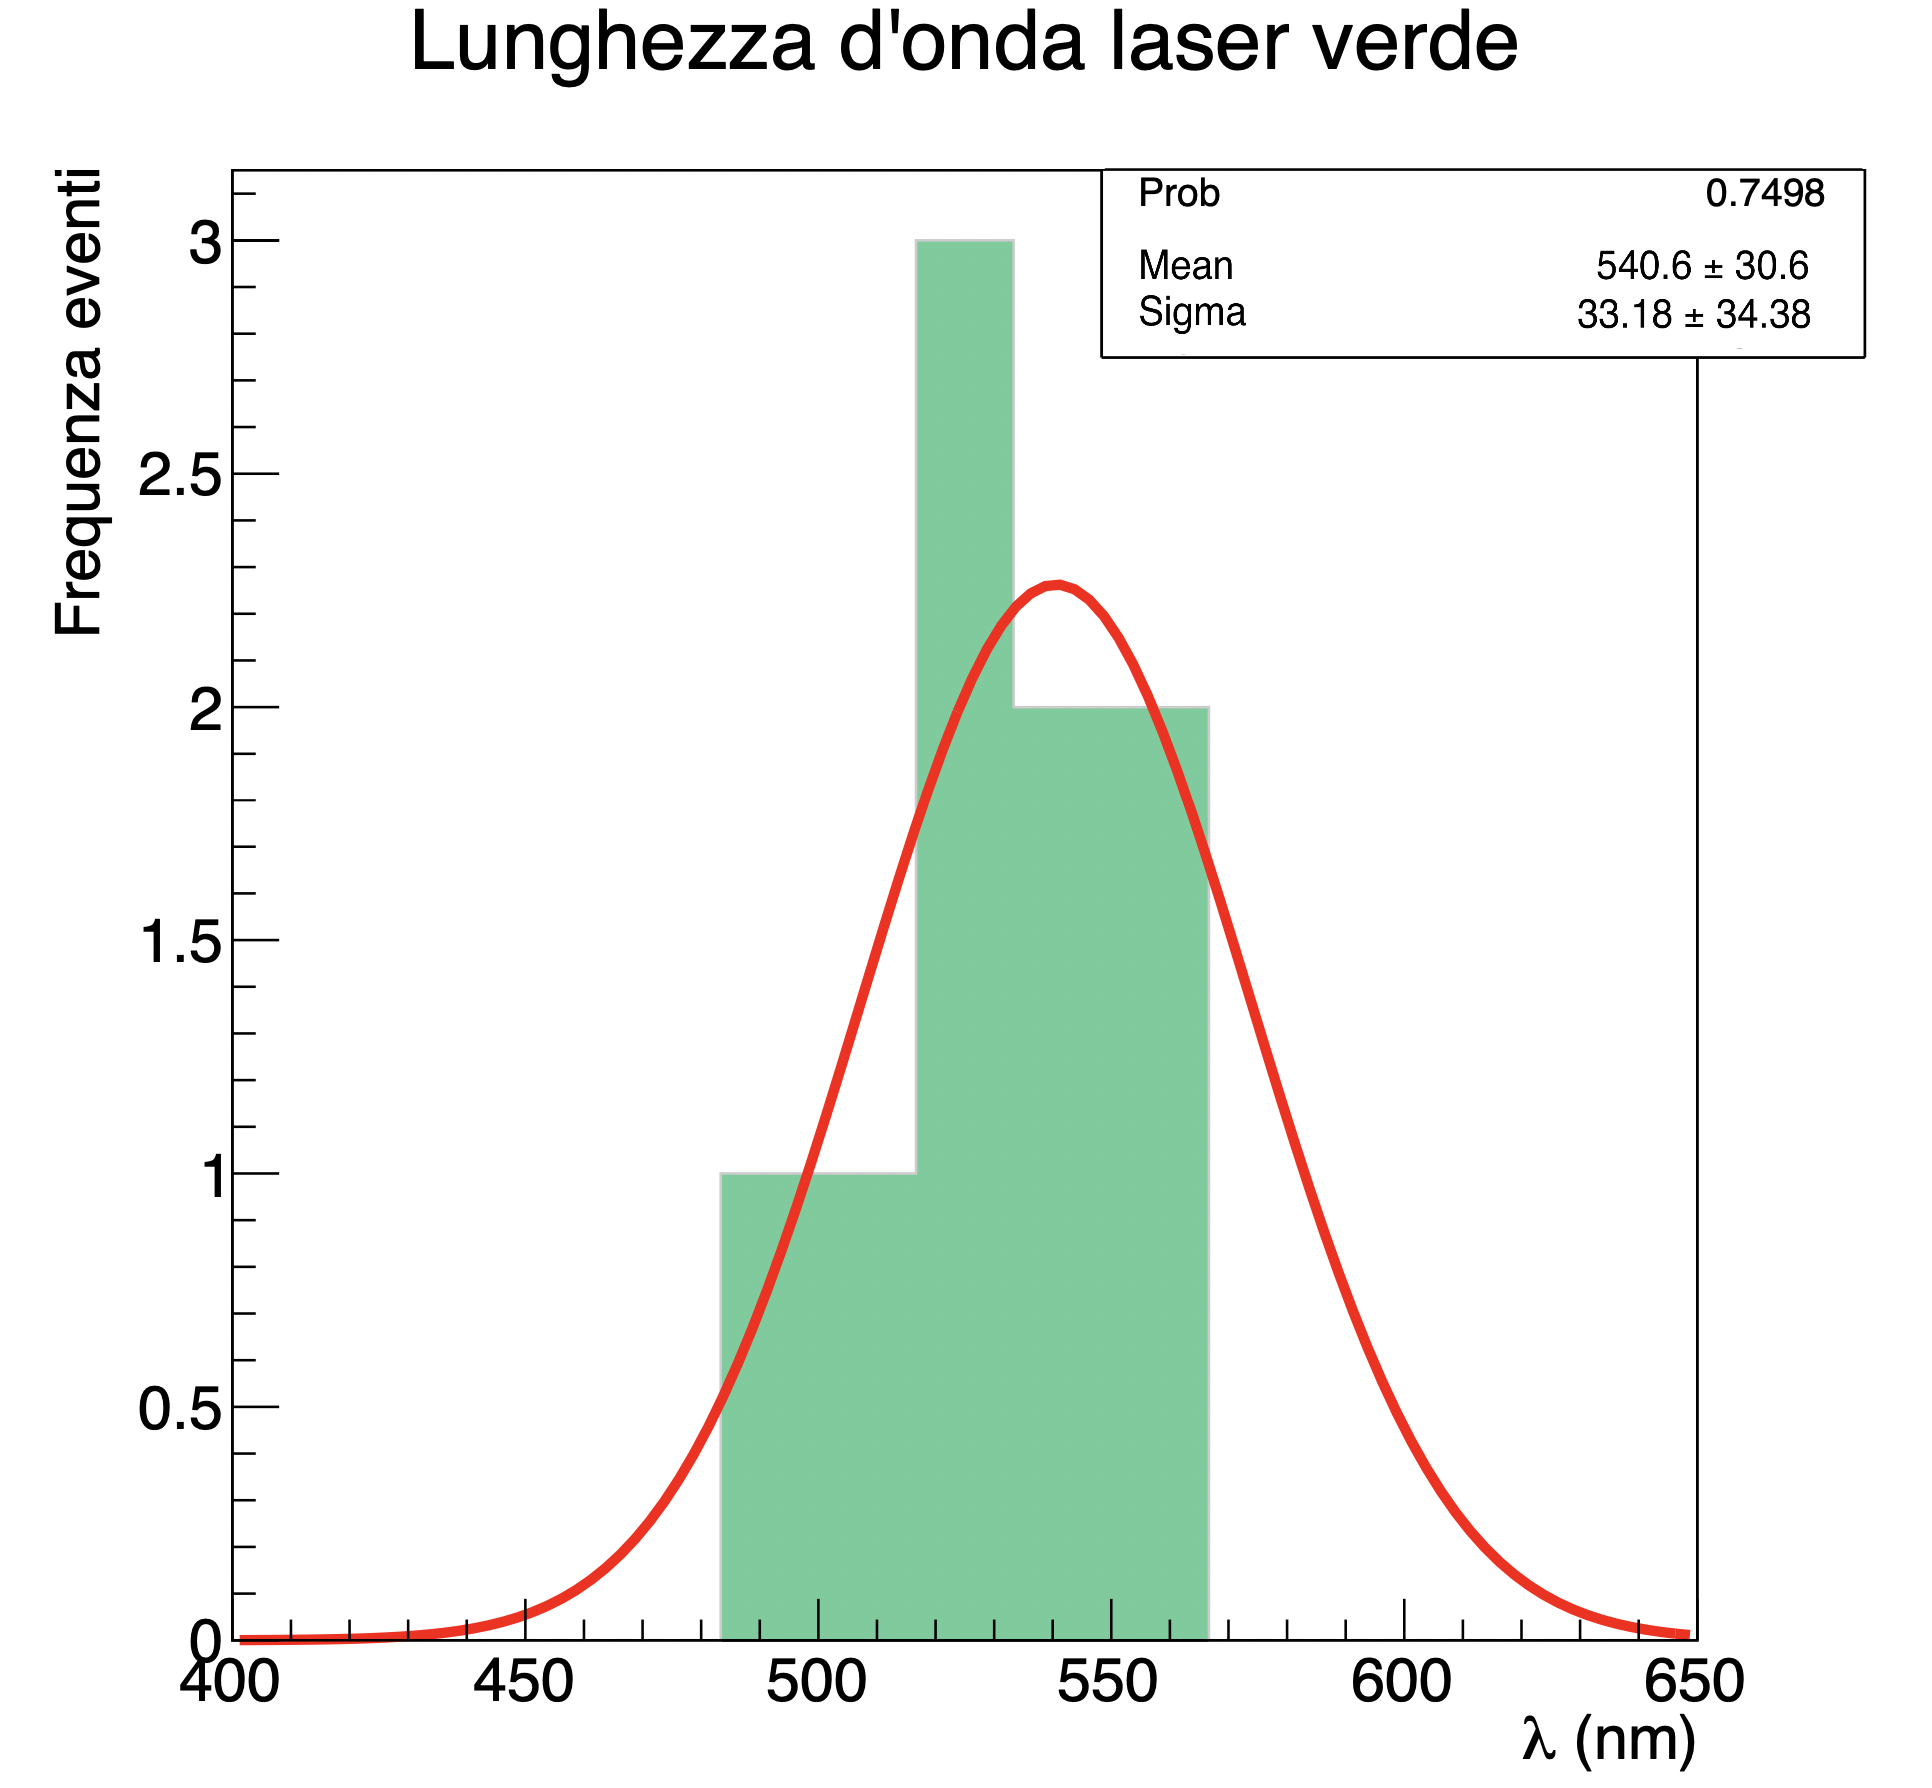
\includegraphics[scale=.33]{immagini/verde.png}
    \caption{}
    \label{fig:my_label}
\end{figure}
Il valore trovato è $\lambda = 534,89\, \pm 23,18\, nm$.












\section{Rifrazione aria}
Dopo aver configurato l'apparato sperimentale per l'esperienza di Michelson, abbiamo inserito la cella con la rispettiva pompa.

Anche in questa parte di esperimento è stato necessario contare il numero di frange, effettuato come in precedenza. 

Abbiamo scelto come zero di pressione la pressione atmosferica e ci siamo mantenuti su variazioni alte di pressione al fine di permettere il conteggio delle frange. Riportiamo i $\Delta P$ facendo notare che il riferimento scelto come zero non incide sui dati raccolti, in quanto differenze di valori, mentre riportiamo in seguito i valori medi per le diverse pressioni:
\FloatBarrier
\begin{table}[h!]
\centering
\begin{tabular}{lccccl}
$\Delta P$ (kPa) & \multicolumn{3}{c}{$\Delta N$} &\quad  \overline{\Delta N}\\ \hline 
80            & 17      & 20      & 17      & 18 \\
70            & 16      & 15      & 15      &  15 \\
60            & 13      & 13      & 13      &  13 \\ 
50            & 10      & 10      & 10      &  10 \\
40            & 8       & 8       & 8       & 8 \\ 
\hline\hline
\end{tabular}
\label{tabella 3}
\caption{}
\end{table}
\FloatBarrier
\noindent
Seguendo la relazione \ref{aria} abbiamo eseguito un'interpolazione lineare dei  $\Delta P$ in funzione dei  $\overline{\Delta N}$ ricavando i parametri:
$$
a = 9,045\,\pm 3,352 \qquad    b = 3,981\, \pm 0,252
$$
Tale scelta è stata fatta per permettere di ricavare gli errori su  $a$ e  $b$, utilizzando come errore per le \textit{y} la precisione dello strumento, cioè  $2\,\operatorname{kPa}$. Dai parametri della retta di interpolazione, in particolar modo dal coefficiente angolare, ci è stato quindi possibile ricavare una stima sperimentale dell'indice di rifrazione dell'aria che risulta essere pari a 
$$
\eta_{\text {aria }}= 1,013 \pm 0,252
$$

\begin{figure}[h!]
    \centering
    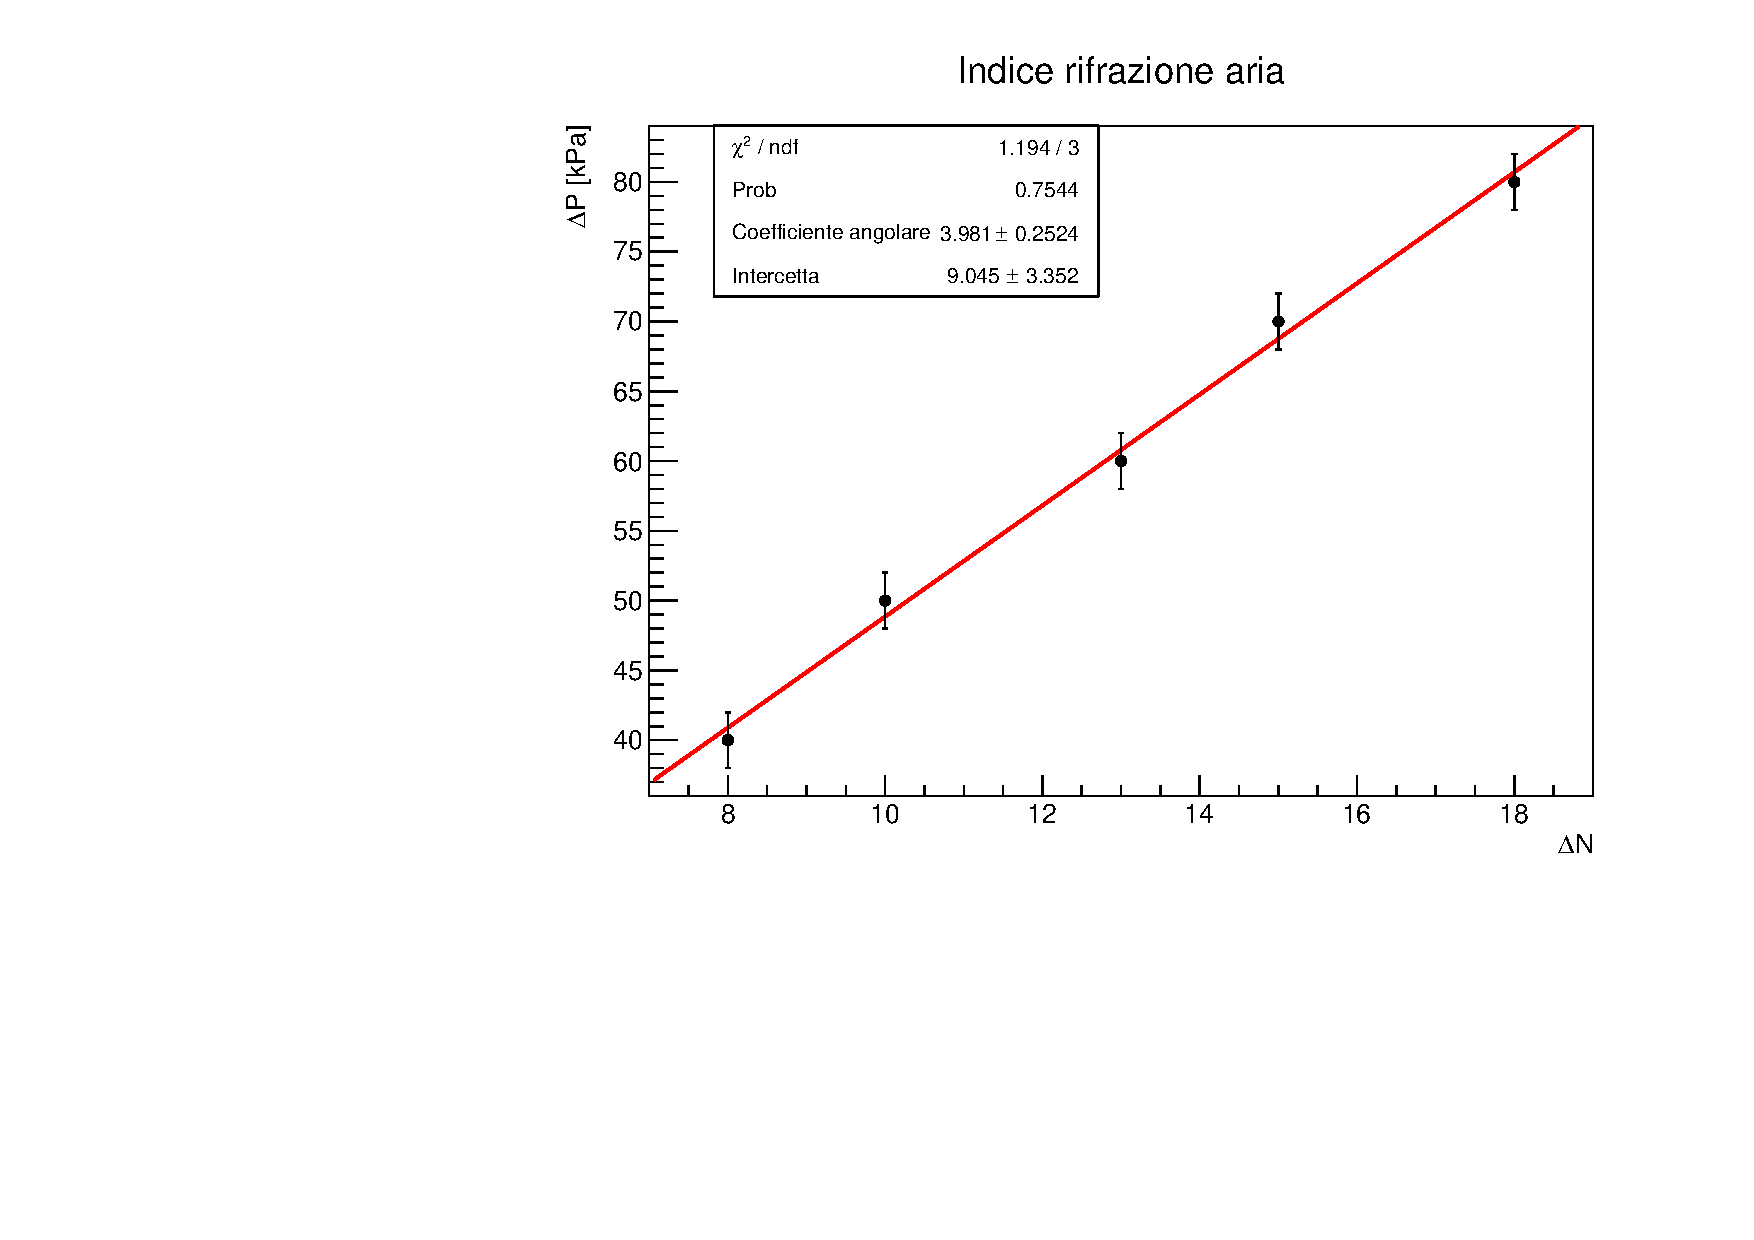
\includegraphics[scale=.6]{immagini/coefficiente aria.pdf}
    \caption{}
    \label{fit aria}
\end{figure}
\section{Rifrazione vetro}
L'ultima misurazione aveva come obiettivo quello di determinare l'indice di rifrazione del vetro; anche in questo caso è stato necessario contare il numero di frange passanti per un riferimento scelto, movimento delle quali causate da un componente aggiuntivo.

Tale componente, sul quale è montata una lastra di vetro, permette il cambiamento della figura di interferenza attraverso la rotazione della lastra stessa. Prima di iniziare l'esperimento è stato necessario determinare l'angolo di inversione, nel nostro caso $\theta = 0,2 \, ^\circ$, che determina il punto in cui le frange invertono il loro moto. 

Per una rotazione di $5 \, ^\circ$ abbiamo ricavato diversi $\Delta N$, riportati di seguito con il relativo istogramma:

\FloatBarrier
\begin{table}[h!]
    \centering
    \begin{tabular}{ccc}
    &\Delta N\\
    \hline
         & 23 & 24 \\
         & 23 & 24 \\
         & 22 & 21 \\ 
         & 25 & 25 \\
         & 23 & 23 \\
    \hline\hline
    \end{tabular}
    \caption{}
\end{table}
\begin{figure}[h!]
    \centering
    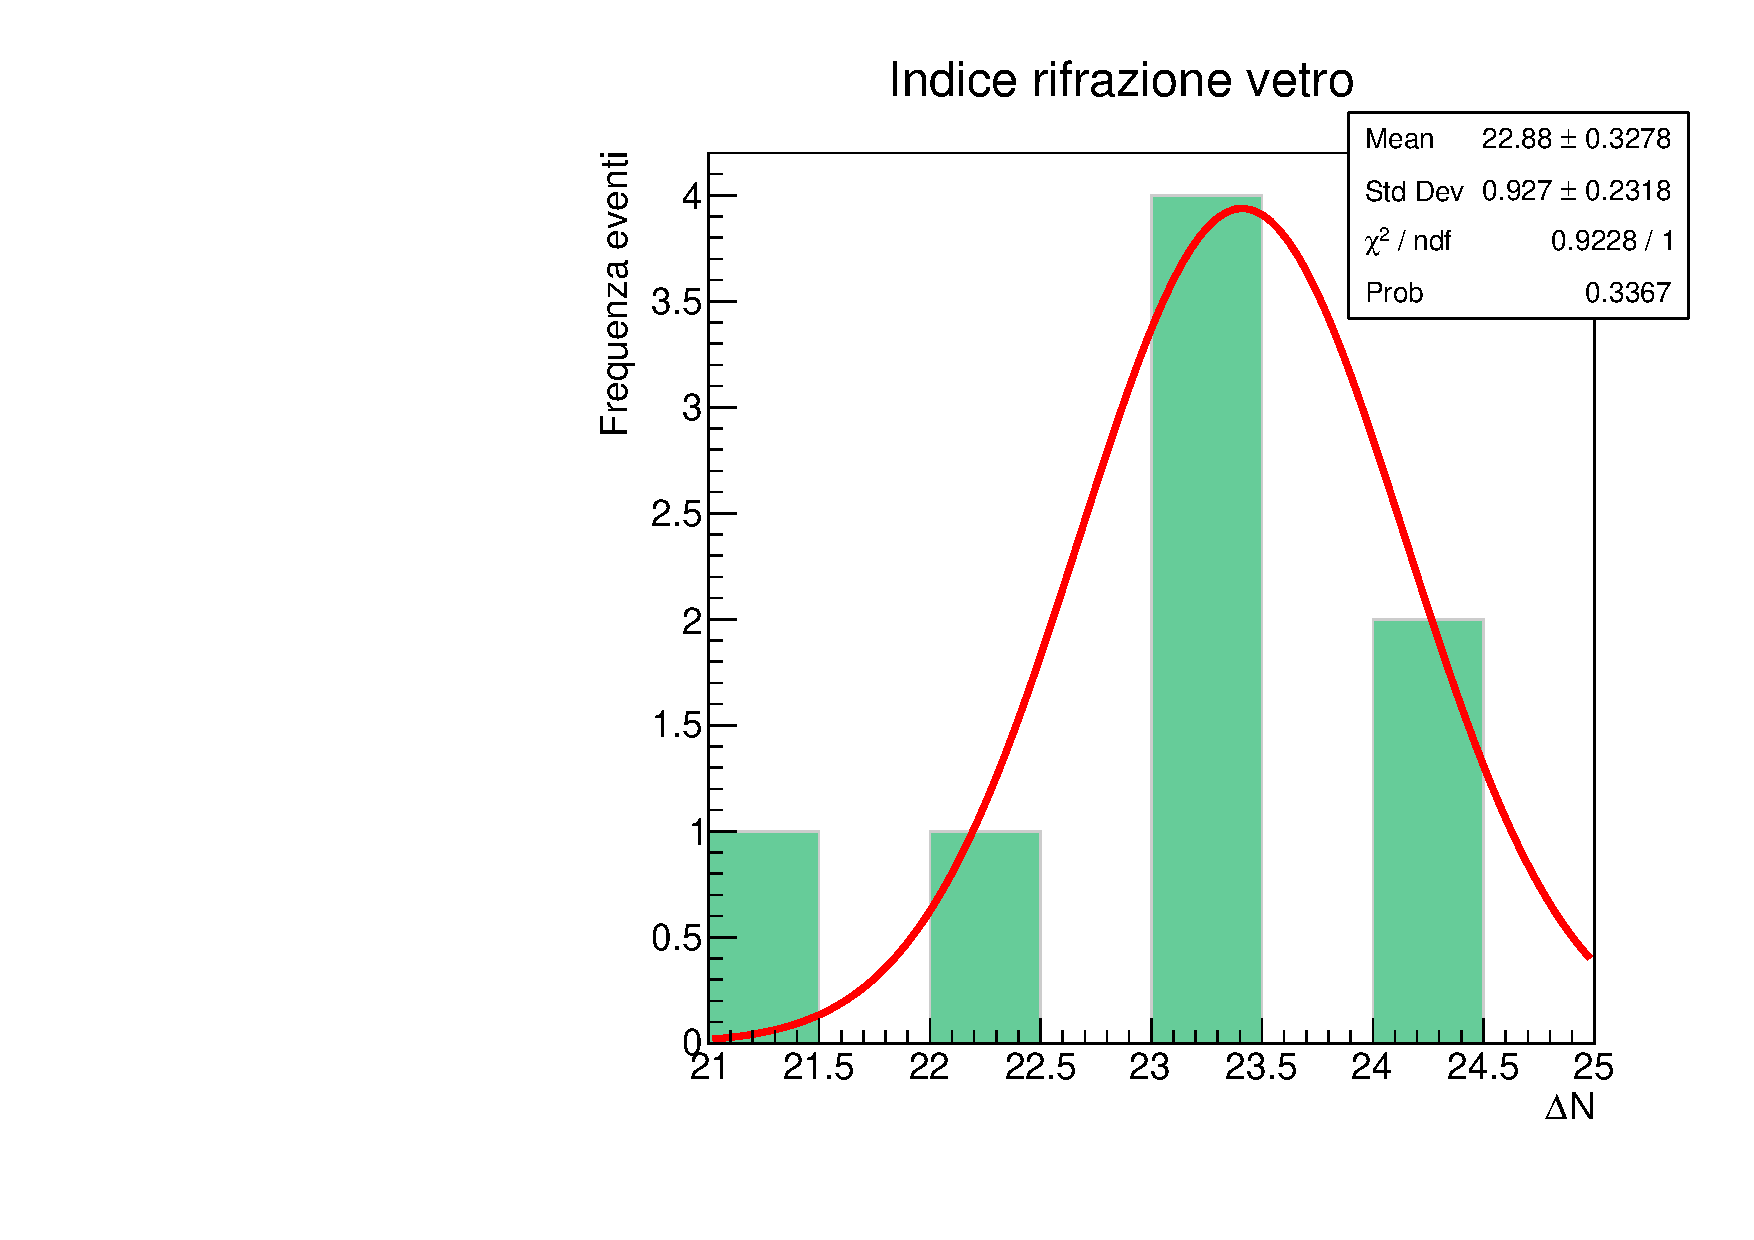
\includegraphics[scale=.4]{immagini/vetro.pdf}
    \caption{}
    \label{fit vetro}
\end{figure}
\FloatBarrier

Dopo aver ripetuto più volte la misura di \textit{d}, riportiamo i dati in tabella, abbiamo ricavato il valore medio di $d = 0,57\, \pm 0,006\, \operatorname{cm}$
\FloatBarrier
\begin{table}[h!]
    \centering
    \begin{tabular}{ccc}
    &\textit{d}\,(cm)\\
    \hline
         & 0.576 \\
         & 0.561 \\
         & 0.571 \\ 
         & 0.571 \\
         & 0.573 \\
    \hline\hline
    \end{tabular}
    \caption{}
\end{table}
\FloatBarrier
Utilizzando, quindi, il valore per \textit{d} trovato e le misure di $\Delta N$, attraverso l'Eq. \ref{eq 3}, abbiamo ricavato i seguenti valori

\FloatBarrier
\begin{table}[h!]
    \centering
    \begin{tabular}{ccc}
    &$n_{\text {vetro }}$ \\
    \hline
        & 1,495  & 1,528\\
        & 1,495  & 1,528\\
        & 1,464  & 1,433\\  
        & 1,563  & 1,563\\
        & 1,495  & 1,495\\
    \hline\hline
    \end{tabular}
    \caption{}
\end{table}
\FloatBarrier
\noindent
\begin{figure}[h!]
    \centering
    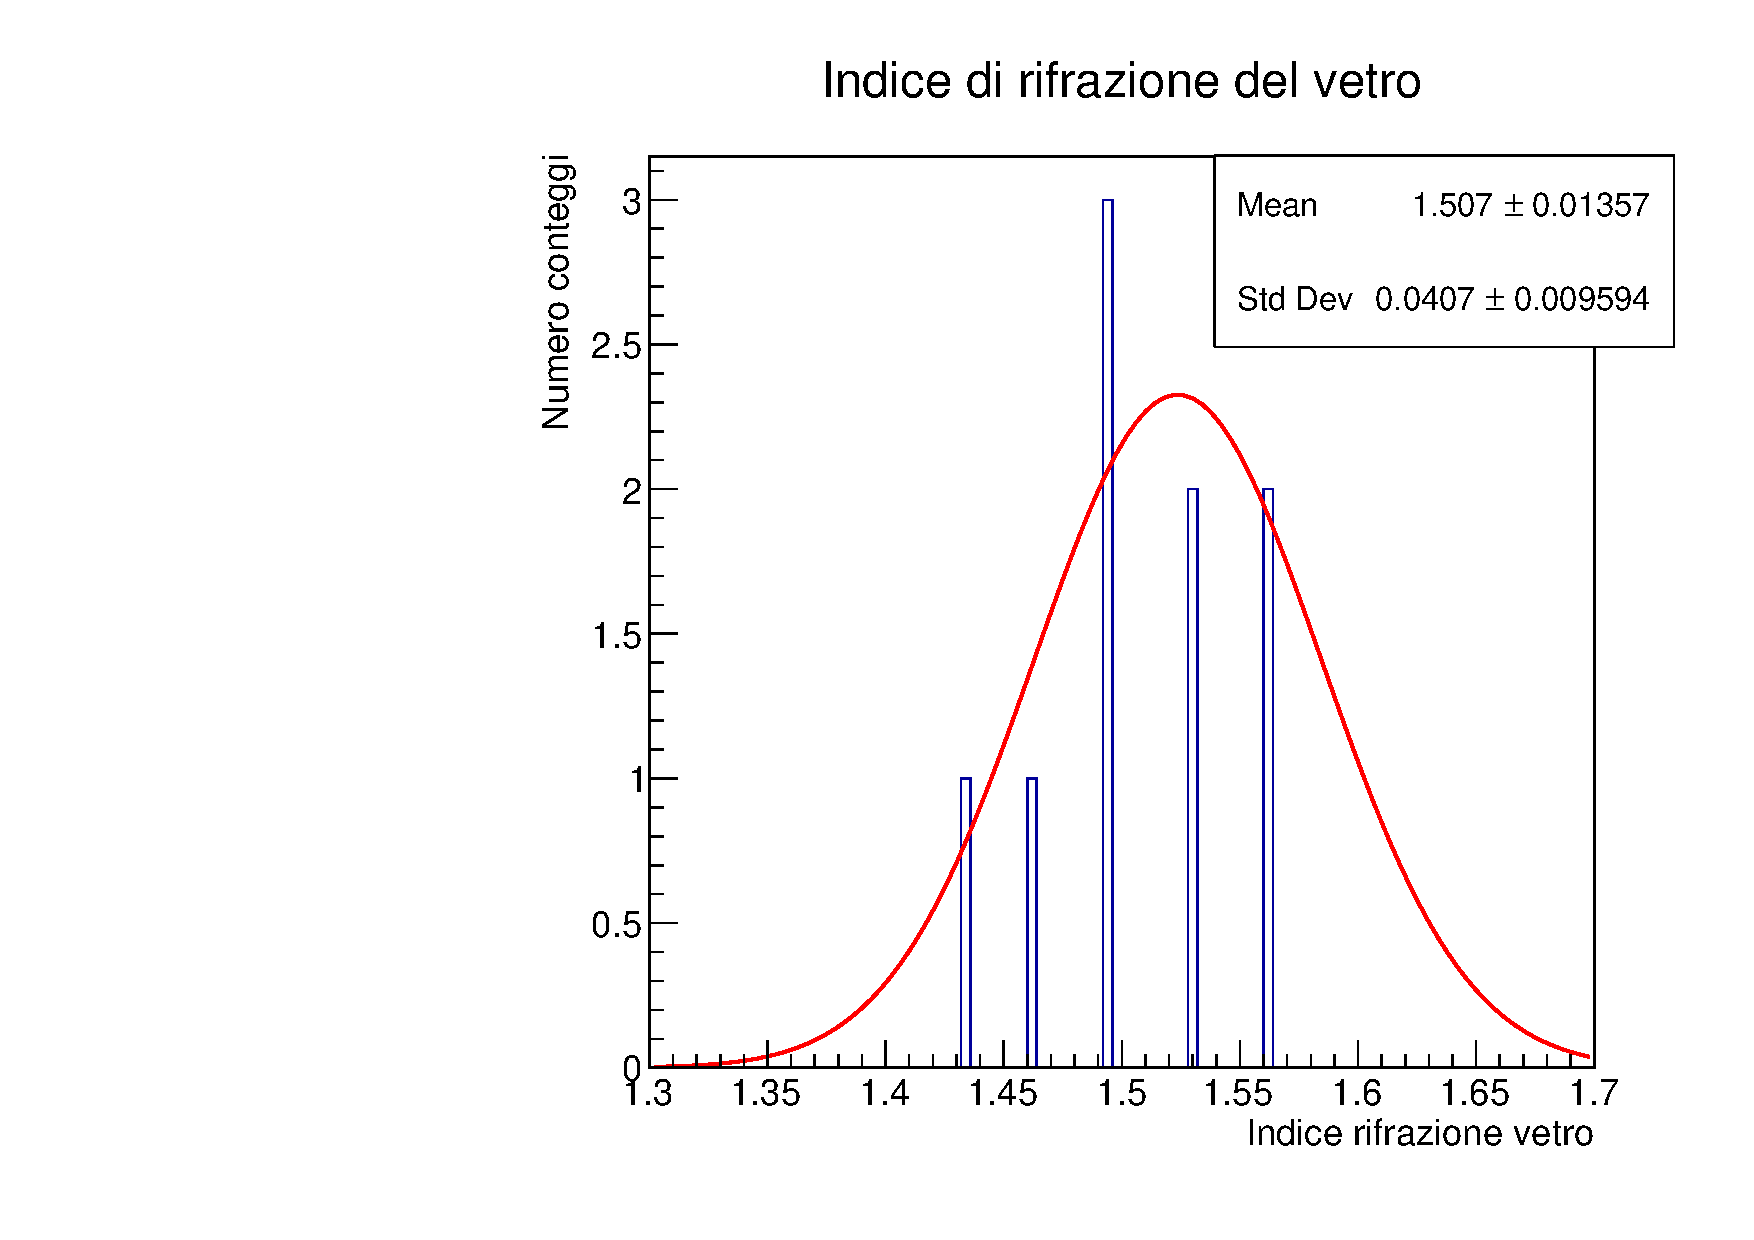
\includegraphics[scale=.4]{immagini/vetro copia.pdf}
    \caption{}
    \label{fig:my_label}
\end{figure}
Infine abbiamo dunque ottenuto il valore del coefficiente di rifrazione del vetro pari a 
$$
\eta_{\text{vetro}}=1,507\pm0,013
$$



%\section{Esperienza virtuale}
Abbiamo infine condotto nuovamente in maniera virtuale la calibrazione e la misura delle lunghezze d'onda di laser di diversi colori, attraverso l'utilizzo di un programma online. I diversi valori attesi per i $\Delta d$ sono riportati di seguito:

\FloatBarrier
\begin{table}[h!]
\centering
\begin{tabular}{lccccl}
$\Delta d$ misurato (\mu m) & $\Delta N$ &  $\Delta d\,\,\text{ricavato}$ (\mu m)\\ \hline 
13            & 43      & 15,69       \\
10            & 33      & 12,04      \\
7            & 23      & 8,39     \\ 
4            & 13      & 4,74       \\
2            & 7       & 2,55        \\ 
\hline\hline
\end{tabular}
\label{tabella 4}
\caption{}
\end{table}
\FloatBarrier
\noindent

Abbiamo utilizzato uno spostamento $\Delta d$ corrispondente a $13\,\mu m$ e abbiamo usato il valore calcolato nella calibrazione, cioè $15,69 \, \mu m$, per ottenere le lunghezze d'onda di laser di diversi colori.
Per il laser giallo abbiamo ricavato un numero di frange pari a:
\begin{table}[h!]
    \centering
    \begin{tabular}{ccc}
    &$\Delta N$\\
    \hline
         &47 &47\\
         &47 &46\\
         &47 &47\\
         &48 &47\\
         &47 &47 \\
         &47 &47 \\
         &48 &47 \\
         &47 &47 \\
    \hline\hline
    \end{tabular}
    \caption{}
\end{table}
\noindent

\begin{table}[h!]
    \centering
    \begin{tabular}{ccc}
    &\lambda\,nm\\
    \hline
         & 578,21 & 578,21 \\
         & 578,21 & 590,78 \\
         & 578,21 & 578,21 \\ 
         & 566,17 & 578,21 \\
         & 578,21 & 578,21 \\
         & 578,21 & 578,21 \\
         & 566,17 & 578,21 \\
         & 578,21 & 578,21 \\
    \hline\hline
    \end{tabular}
    \caption{}
\end{table}
\FloatBarrier
\noindent

Il valore ottenuto è quindi $\lambda = 578,28
\, \pm 60,44\, nm$ 

Per il laser azzurro abbiamo ottenuto questi dati:
\begin{table}[h!]
    \centering
    \begin{tabular}{ccc}
    & Numero di frange $\Delta N$\\
    \hline
         &52 &52\\
         &51 &52\\
         &52 &52\\
         &52 &53\\
         &53 &52 \\
         &52 &52 \\
         &52 &51 \\
         &53 &52 \\
    \hline\hline
    \end{tabular}
    \caption{}
\end{table}
\noindent

\begin{table}[h!]
    \centering
    \begin{tabular}{ccc}
    &\lambda\,nm\\
    \hline
         & 522,62 & 522,62 \\
         & 532,86 & 522,62 \\
         & 522,62 & 522,62 \\ 
         & 522,62 & 512,76 \\
         & 512,76 & 522,62 \\
         & 522,62 & 522,62 \\
         & 522,62 & 532,86 \\
         & 512,76 & 522,62 \\
    \hline\hline
    \end{tabular}
    \caption{}
\end{table}
\FloatBarrier
\noindent

Il valore ottenuto è quindi $\lambda = 522,05\, \pm 54,57\, nm$ 

Per il laser verde abbiamo ottenuto questi dati:
\begin{table}[h!]
    \centering
    \begin{tabular}{ccc}
    & Numero di frange $\Delta N$\\
    \hline
         & 60 & 61\\
         &60 &60\\
         &62 &59\\
         &60 &62\\
         &60 &60 \\
         &61 &60 \\
         &60 &60 \\
         &62 &61 \\
    \hline\hline
    \end{tabular}
    \caption{}
\end{table}
\noindent

\begin{table}[h!]
    \centering
    \begin{tabular}{ccc}
    &\lambda\,nm\\
    \hline
         & 452,93 & 445,51 \\
         & 452,93 & 452,93 \\
         & 438,32 & 460,61 \\ 
         & 452,93 & 438,32 \\
         & 452,92 & 445,51\\
         & 452,93 & 452,93 \\
         & 445,51 & 438,32 \\
    \hline\hline
    \end{tabular}
    \caption{}
\end{table}
\FloatBarrier
\noindent

Il valore ottenuto è quindi $\lambda = 449,28
\, \pm 46,96\, nm$ 

In tutti casi abbiamo ottenuto dei valori che rientrano nell'intervallo di spettro di luce visibile corrispondente al colore dato.



\section{Conclusioni}
Lo scopo dell'esperimento era quello di misurare, attraverso il fenomeno dell'interferenza, diverse quantità.
E' importante notare come la calibrazione ci abbia permesso di ottenere misure più precise e più accurate; l'accuratezza, in particolar modo, ci ha permesso di limitare i bias sui valori ottenuti. Tale risultato è stato reso manifesto dalla misura ricavata per la lunghezza d'onda  del laser verde, la quale rientra nell'intervallo di spettro che corrisponde a quel colore. 
Diversi erano, invece, gli obiettivi utilizzando l'apparato di Michelson; in entrambi i casi gli esperimenti sono stati soddisfacenti, come mostrano i valori per i due \textit{t-test}.

Nella misura dell'indice di rifrazione dell'aria dal \textit{t-test} si ricava un valore di $0,05\, \sigma $; il motivo di un valore così basso può essere dovuto a una sovrastima dell'errore, oppure causato dal fatto che il valore vero dell'indice di rifrazione dell'aria scelto per fare il t-test non corrisponda a quello reale, influenzato dalla temperatura e dalla pressione presente in laboratorio. Il valore del \textit{t-test} per l'indice di rifrazione del vetro è $0,51\,\sigma $, il quale risulta coerente con le misurazioni prese. 

I risultati dell'esperimento portano, quindi, alla conclusione che entrambi i sistemi ottici siano validi per condurre esperimenti riguardanti il fenomeno dell'interferenza della luce. Tuttavia mostrano come che per misure come quella dell'indice di rifrazione dell'aria siano necessari strumenti più precisi e uno studio più approfondito delle condizioni dell'ambiente in laboratorio.


\end{document}